This section describes the background estimation methods used in the HH analysis. 

The simulated event samples summarised in Section~\ref{sec:data_backgrounds} are used to model all background processes, except for processes with fake-\tauhad\ which are estimated using data-driven techniques, as discussed below. In the \lephad channel, all fake-\tauhad\ backgrounds from $t\bar{t}$ and multi-jet processes are estimated using an inclusive fake-factor method, described in Section~\ref{subsec:LepHadfake}. In the \hadhad channel, the multijet background is estimated using a data-driven fake-factor method as described in Section~\ref{subsec:HadHadmultijet} and the $t\bar{t}$ background with fake-\tauhad\ is estimated using a scale-factor method with scale-factors derived from data to correct the MC prediction as described in Section~\ref{sec:ttbarfake_hadhad_sf_method}.


% The \ttbar\ with true-\tauhad\ and Z+HF templates are taken from the MC prediction
%  but their normalisations are derived from data as included as freely floating parameters in the final fit,
%   as described in Section~\ref{sec:fit}. 

Events with electrons or muons that are misidentified as \tauhad\ objects, 
dominantly coming from the \ttbar\ production, 
represent a minor background in the analysis and they are estimated from simulation. 
This background is treated together with the 
\ttbar\ events containing true-\tauhad\ objects. 
% Additional material can be found in Appendix~\ref{subsec:appendix_bkg_leptons_faking_taus}.


\subsection{Fake-$\tau$ backgrounds in the \lephad channel}
\label{subsec:LepHadfake}

Background processes where a jet is misidentified as a \tauhad, 
referred to as fake-\tauhad\ processes, 
are estimated using a data-driven method due to imperfect MC modelling of these processes.
Feynman diagrams in Figure~\ref{fig:fakes:feynman} 
show examples of the two dominant processes contributing to the fake-\tauhad\ background,
which are \ttbar\ and multi-jet (QCD) processes. 
In \ttbar\ events, the fake-\tauhad\ typically originates from quark initiated jets from 
top-quark decay; in multi-jet events jets initiated from both quark and gluon can be
misidentified as \tauhad. 
\begin{figure}[htbp]
\centering
\includegraphics[width=.45\textwidth]{DiHiggs/plots/lephadFF/SLT/2tag2pjet_0ptv_HighMtCR_TauPt150_CR_SLT_ALL_ttWeight_1.png}
\caption{Plots of the $\tauhad$ $p_T$ distributions for the (left) anti-\tauhad\ and (right) \tauhad\ selection for the (top) single lepton trigger and (bottom) lepton-plus-tau trigger selections in the \ttbar\ control region with 1-prong \tauhad.}
\label{fig:fakes:feynman}
\end{figure} 

The strategy for estimating such background is based on the `fake factor' (FF) method.
The FF is a measure of the ratio of the number of signal region events with a fake-\tauhad, 
(fake-\tauhad\ events)
to the number of control region events with a fake-\tauhad.
In the case of the \bbtautau\ channel, a fake-\tauhad\ enriched region is provided by the
anti-\tauhad\ selection (anti-\tauhad\ region),   
as defined in Section~\ref{} TODO: add reference to antitau selection.
In the case where the event contains more than one anti-\tauhad, 
one is chosen randomly. Derived variables used in the analysis,
such as the \MET, $m^{\mathrm{MMC}}_\mathrm{T}$ and \MET$\phi$ centrality 
are calculated in the same way as for signal events, 
but with the anti-\tauhad\ taking the place of the loose \tauhad\ candidate.
% The anti-\tauhad\ selection provides a region with enriched fake-\tauhad\ events,
% and hence one can extrapolate the fake-\tauhad\ background events from the 
% fake-\tauhad\ enriched region to the signal region 
% once the fake factor is estimated properly.
% Given that, 
Given that, the fake factor is calculated as:
\begin{equation}
	\mathrm{FF} =  \frac{N(\text{loose }\tauhad)}{N(\mathrm{anti}\mhyphen\tauhad)} 
\end{equation} 
where $N(\text{loose }\tauhad)$ ($N(\mathrm{anti}\mhyphen\tauhad)$) is the number of 
data events with a nominal \tauhad\ (anti-\tauhad) with 
contributions from true \tauhad\ subtracted from each term.
Due to the different origins of the fake-\tauhad, the FF are
calculated separately for \ttbar\ and multi-jet, and for 1 and 3-prong \tauhad\ candidates.
For each process the $FF$ are calculated in a dedicated background enriched region. 
The control regions for each process are defined as follows:
 \begin{itemize}
	\item \ttbar\ CR: \mbb\ > 150 GeV, 2 $b$-tag 
 	\item Multi-jet (QCD) CR: inverted lepton isolation 
	 (`tight' electrons and `medium' muons are 
	 required to fail their respective `loose' isolation working points), 
	 2 $b$-tag. 
 \end{itemize}



 Individual fake-factors for each process
 are then used to provide a combined fake-factor. 
 The combined $FF$ is then applied to the anti-\tauhad\ events 
 in order to extrapolate to the SR which gives an estimation
 of the fake-\tauhad\ events in the SR.
 The combined fake-factor is defined as:
 
 \begin{equation}
 FF(\mathrm{comb}) = FF(\mathrm{QCD}) \times \mathrm{r}_{\mathrm{QCD}} + FF(\ttbar) \times (1 - \mathrm{r}_{\mathrm{QCD}}) 
 \end{equation} 
 
 where $\mathrm{r}_{\mathrm{QCD}}$ is measured as a function of the \tauhad\ \pT\ 
 and defined as the fraction of multi-jet events in the anti-tau signal region:
 
 \begin{equation}
 \mathrm{r}_{\mathrm{QCD}} = \frac{N(\mathrm{multi\mhyphen jet, data})} {N(\mathrm{data}) - N(\mathrm{true}~\tauhad, \mathrm{MC})}
 \end{equation} 
 where the $N(\mathrm{multi\mhyphen jet, data})$ is calculated by 
 subtracting all background contributions apart from multi-jet, 
 regardless of whether they contain fake or true-\tauhad\ candidates, 
 from the data in the anti-\tauhad\ selection:
 \begin{equation}
	 N(\mathrm{multi\mhyphen jet, data}) = N(\mathrm{data}) - N(\mathrm{true}~\tauhad, \mathrm{MC} + \mathrm{fake}~\tauhad, \mathrm{MC})
 \end{equation}  
 The subtracted backgrounds are taken from the MC predictions. 
 In graphical form, the various control regions 
 where the fake factors are measured and applied can be seen in Figure~\ref{fig:CombFFMethod}.
 \begin{figure}
 \centering
 \includegraphics[width=.9\textwidth]{DiHiggs/plots/FF regions.png}
 \caption{Graphical representation of the Combined Fake Factor Method. 
 The fake factors are calculated independently for the \ttbar\ CR and the multi-jet CR, and 
 combined to the combined fake factor. 
 The direction of the arrow indicates the direction 
 of extrapolation when applying the fake factor.}
 \label{fig:CombFFMethod}
 \end{figure}
The fake factor is parameterized in \pt\ of the \tauhad, where it shows an obvious trend.
The depending on $\eta$ of the \tauhad\ is also checked but no clear trend is found, as shown in 
Figure~\ref{fig:lhFF_eta_SLT}, \ref{fig:lhFF_eta_LTT} for the SLT and LTT channels respectively.  


\begin{figure}
\centering
\includegraphics[width=.4\textwidth]{DiHiggs/plots/lephadFF/SLT/FF_All_Preselection_Np1_HighMtCR_2tag_Tau0Eta}
\includegraphics[width=.4\textwidth]{DiHiggs/plots/lephadFF/SLT/FF_All_Preselection_Np3_HighMtCR_2tag_Tau0Eta}\\
\includegraphics[width=.4\textwidth]{DiHiggs/plots/lephadFF/SLT/FF_All_Preselection_Np1_CR_2tag_Tau0Eta}
\includegraphics[width=.4\textwidth]{DiHiggs/plots/lephadFF/SLT/FF_All_Preselection_Np3_CR_2tag_Tau0Eta} \\
\caption{Fake-factors as a function of $\eta$ for 1-prong (left) and 3-prong (right) \tauhad\ candidates for \ttbar\ CR (top) 
and multi-jet (bottom) for the \lephad SLT category. No significant trend is observed.}
\label{fig:lhFF_eta_SLT}
\end{figure}

\begin{figure}
\centering
\includegraphics[width=.4\textwidth]{DiHiggs/plots/lephadFF/LTT/FF_All_Preselection_Np1_HighMtCR_2tag_Tau0Eta}
\includegraphics[width=.4\textwidth]{DiHiggs/plots/lephadFF/LTT/FF_All_Preselection_Np3_HighMtCR_2tag_Tau0Eta}\\
\includegraphics[width=.4\textwidth]{DiHiggs/plots/lephadFF/LTT/FF_All_Preselection_Np1_CR_2tag_Tau0Eta}
\includegraphics[width=.4\textwidth]{DiHiggs/plots/lephadFF/LTT/FF_All_Preselection_Np3_CR_2tag_Tau0Eta} \\
\caption{Fake-factors as a function of $\eta$ for 1-prong (left) and 3-prong (right) \tauhad\ candidates for \ttbar\ CR (top) 
and multi-jet (bottom) for the \lephad LTT category. No significant trend is observed.}
\label{fig:lhFF_eta_LTT}
\end{figure}

The determination of the combined fake factor 
is sensitive to the modelling of simulated $t\bar{t}$ events with true-\tauhad\
given that this is the dominant background that is subtracted from data in the derivation of
the FFs and $\mathrm{r}_\text{QCD}$, and when obtaining the SR Template. Additionally, the derivation
of $\mathrm{r}_\text{QCD}$ is sensitive to the modelling of simulated $t\bar{t}$ events with fake-\tauhad.
It was observed that mismodeling in the \ttbar\ background 
especially in the high jet multiplicity and high top-quark \pt\ region
can cause issues in the calculation of the fake factors, 
giving non-physical negative values at high \tauhad\ \pt\ region. 
To mitigate this issue,
simulated events from $t\bar{t}$ production are differentially reweighted
depending on the jet multiplicity and the scalar sum of the transverse momentum of all visible
final state objects in the event.
These reweighting factors are determined from another $t\bar{t}$ control region ($t\bar{t}$ CR2),
% which is about 93\% pure in the events from $t\bar{t}$ production,
which is defined using a selection identical to the SR selection,
but with the \ttbar\ CR $m_{bb}$ requirements ($m_{bb}>150$~GeV)
and an additional $m^{W}_\text{T}>40$~GeV requirement. 
Furthermore, events in this control region are required
to have a reconstructed \tauhad\ candidate, but this candidate is not required
to pass the RNN \tauhad\ identification criteria defined in Section~\ref{sec:rec:tau}.
The $m^{W}_\text{T}$ requirement is introduced to remove any potential contamination from multi-jet events.
The reweighting method is validated in two additional validation region, as described in more details in
Appendix~\ref{} TODO: add reference to appendix. 
The reweighting only applies to the control regions and the anti-\tauhad\ region, 
while it's not necessary applying to the signal region 
where it would complicate the \ttbar\ systematics uncertainties and statistical analysis.
The \ttbar\ CR and multi-jet CR events with an anti-\tauhad\ candidate after the \ttbar\ reweighting 
are shown in Figure~\ref{fig:ttbarCR_1}, \ref{fig:ttbarCR_3}, \ref{fig:InvCR_1} and \ref{fig:InvCR_3}.
These plots can also be used to check the purity of the fake-\tauhad\ events in the \ttbar\ and multi-jet CRs,  
where the fakes contributions from \ttbar\ are given from MC simulation.
In the multi-jet control region, the events show large discrepancy between the
data and the MC distributions, as a result of the fakes originating from the 
multi-jet processes which are not simulated by the MC. 
A much larger fraction of \ttbar\ fakes are presented in the \ttbar\ CR. 
The MC does not agree with data very well due to the imperfect \ttbar\ fakes MC simulation,
which is the main motivation for using the data-driven FF method. 

\begin{figure}
\centering
\includegraphics[width=.45\textwidth]{DiHiggs/plots/FF_CRs/ttbarCR_SLT/HNone/BDTVarsHighMbb/2/C_2tag2pjet_0ptv_TauPt1P.png}
\includegraphics[width=.45\textwidth]{DiHiggs/plots/FF_CRs/ttbarCR_LTT/HNone/BDTVarsHighMbb/2/C_2tag2pjet_0ptv_TauPt1P.png}\\
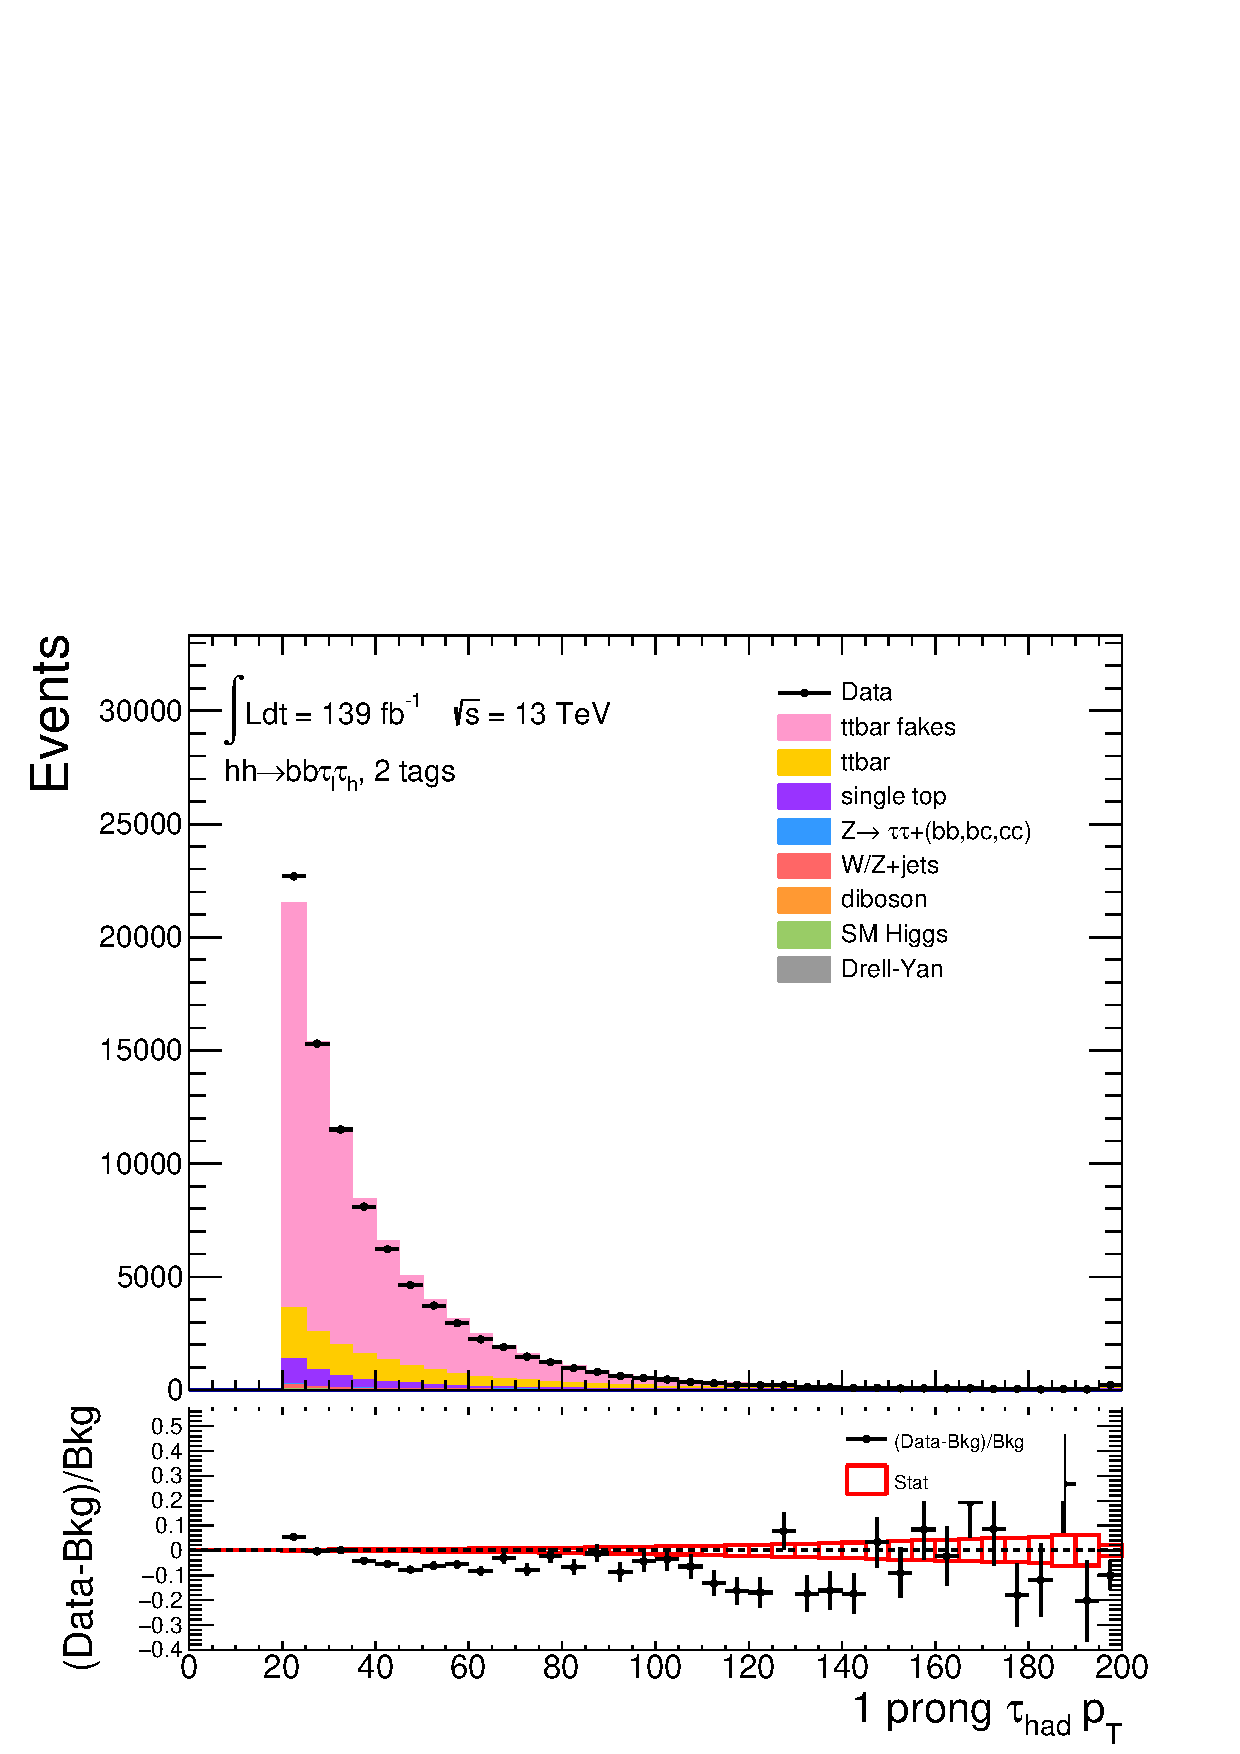
\includegraphics[width=.45\textwidth]{DiHiggs/plots/FF_CRs/ttbarCR_SLT_weighted/HNone/BDTVarsHighMbb/2/C_2tag2pjet_0ptv_TauPt1P.png}
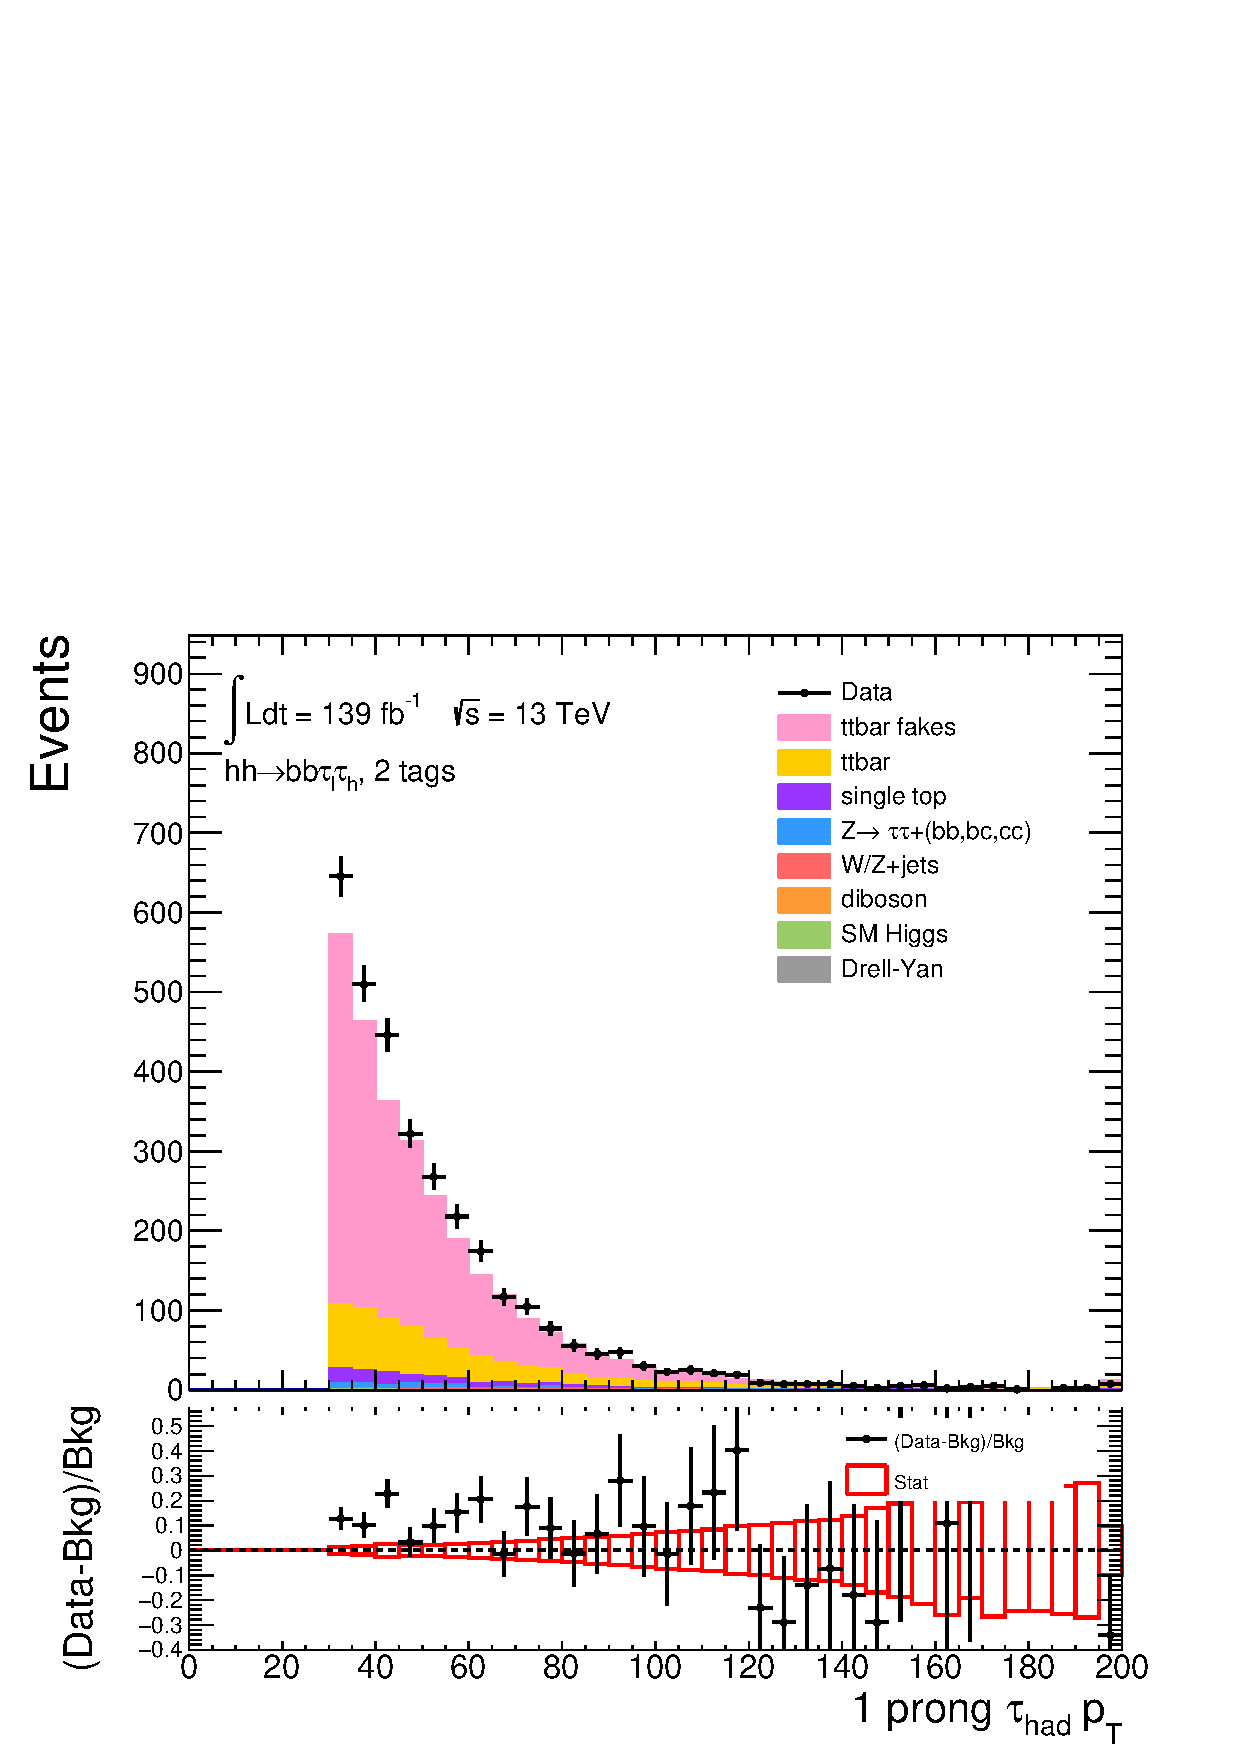
\includegraphics[width=.45\textwidth]{DiHiggs/plots/FF_CRs/ttbarCR_LTT_weighted/HNone/BDTVarsHighMbb/2/C_2tag2pjet_0ptv_TauPt1P.png}\\
\caption{Plots of the $\tauhad$ $p_T$ distributions for the SLT (left) and LTT channel (right) with \ttbar\ un-weighted (top)
and with \ttbar\ re-weighted (bottom) in the \ttbar\ control region with 1-prong anti-\tauhad. 
The \ttbar\ initiated fakes background is labelled as `ttbar fakes' in pink.
With true \tauhad\ contributions subtracted from data (and with true \tauhad\ \ttbar\ reweighted),  
this region is used as the denominator of the \ttbar\ control region fake factor calculation.}
\label{fig:ttbarCR_1}
\end{figure} 
\begin{figure}
\centering
\includegraphics[width=.45\textwidth]{DiHiggs/plots/FF_CRs/ttbarCR_SLT/HNone/BDTVarsHighMbb/2/C_2tag2pjet_0ptv_TauPt3P.png}
\includegraphics[width=.45\textwidth]{DiHiggs/plots/FF_CRs/ttbarCR_LTT/HNone/BDTVarsHighMbb/2/C_2tag2pjet_0ptv_TauPt3P.png}\\
\includegraphics[width=.45\textwidth]{DiHiggs/plots/FF_CRs/ttbarCR_SLT_weighted/HNone/BDTVarsHighMbb/2/C_2tag2pjet_0ptv_TauPt3P.png}
\includegraphics[width=.45\textwidth]{DiHiggs/plots/FF_CRs/ttbarCR_LTT_weighted/HNone/BDTVarsHighMbb/2/C_2tag2pjet_0ptv_TauPt3P.png}\\
\caption{Plots of the $\tauhad$ $p_T$ distributions for the SLT (left) and LTT channel (right) with \ttbar\ un-weighted (top)
and with \ttbar\ reweighted (bottom) in the \ttbar\ control region with 3-prong anti-\tauhad.
The \ttbar\ initiated fakes background is labelled as `ttbar fakes' in pink.
With true \tauhad\ contributions subtracted from data (and with true \tauhad\ \ttbar\ reweighted), 
this region is used as the denominator of the \ttbar\ control region fake factor calculation.}
\label{fig:ttbarCR_3}
\end{figure} 
\begin{figure}
\centering
\includegraphics[width=.45\textwidth]{DiHiggs/plots/FF_CRs/InvCR_SLT/HNone/BDTVarsHighMbb/2/C_2tag2pjet_0ptv_TauPt1P.png}
\includegraphics[width=.45\textwidth]{DiHiggs/plots/FF_CRs/InvCR_LTT/HNone/BDTVarsHighMbb/2/C_2tag2pjet_0ptv_TauPt1P.png}\\
\caption{Plots of the $\tauhad$ $p_T$ distributions for the SLT (left) and LTT channel (right) with \ttbar\ reweighted 
in the multi-jet control region with 1-prong anti-\tauhad. 
The \ttbar\ initiated fakes background is labelled as `ttbar fakes' in pink.
With true \tauhad\ contributions subtracted from data, 
this region is used as the denominator of the \ttbar\ control region fake factor calculation.}
\label{fig:InvCR_1}
\end{figure} 

\begin{figure}
\centering
\includegraphics[width=.45\textwidth]{DiHiggs/plots/FF_CRs/InvCR_SLT/HNone/BDTVarsHighMbb/2/C_2tag2pjet_0ptv_TauPt3P.png}
\includegraphics[width=.45\textwidth]{DiHiggs/plots/FF_CRs/InvCR_LTT/HNone/BDTVarsHighMbb/2/C_2tag2pjet_0ptv_TauPt3P.png}\\
\caption{Plots of the $\tauhad$ $p_T$ distributions for the SLT (left) and LTT channel (right) with \ttbar\ reweighted.
The \ttbar\ initiated fakes background is labelled as `ttbar fakes' in pink.
With true \tauhad\ contributions subtracted from data, 
this region is used as the denominator of the multi-jet control region fake factor calculation.}
\label{fig:InvCR_3}
\end{figure} 

The calculated fake factors are shown on Figure~\ref{fig:SLT_FF} and Figure~\ref{fig:LTT_FF}, 
for the SLT and LTT channels respectively. 
The Fake factors obtained with reweighted and un-weighted \ttbar\ contributions are shown on the
same graph. 
The binning is optimised for the $\text{FF}_{t\bar{t}}$ and the same binning is used for the 
$\text{FF}_\text{QCD}$. As a result a smooth trend is observed in the $\text{FF}_{t\bar{t}}$ 
but some artifacts shapes at mid and high \pt\ range are showin in the $\text{FF}_\text{QCD}$.
This issue has no visible impact on the fakes estimation, because the 
the \ttbar\ FF dominates over the multi-jet FF in the combined FF which can be seen 
in the $\mathrm{r}_\text{QCD}$ distribution in the following. 
% It was observed that known mismodeling in the \ttbar\ 
% background can cause issues in the calculation of the fake factors, 
% most notably making them eventually become negative at very high values of $\tau$ transverse momentum.  
% For this reason, the \ttbar\ background is reweighted 
% when it is subtracted in the calculation and application of fake factors.  
% This reweighting method is described in Appendix~\ref{subsec:appendix_bkg_ttbar_reweighting}.  
% The difference between the background estimation achieved with and without this \ttbar\ reweighting 
% will be taken as an additional uncertainty on the method. The FF comparison 
% with \ttbar-reweighting vs. no-\ttbar-reweighting is shown 
% in Fig. \ref{fig:FFRW} for a demonstration of this uncertainty. 
% This reweighting is applied in all the control regions used for the calculation 
% of the combined fake factors, though it has the largest impact on the \ttbar\ fake factor contribution. 
The $\mathrm{r}_{\mathrm{QCD}}$ is computed both for $e\tauhad$ and $\mu\tauhad$ channels, 
since the QCD contents are different for them.
The parameterized $\mathrm{r}_{\mathrm{QCD}}$ 
as a function of \pT(\tauhad) for 1-prong and 3-prong \tauhad\ candidates in $e\tauhad$ and $\mu\tauhad$ channels 
are shown in Figure~\ref{fig:SLT_rQCD} for the SLT category and 
in Figure~\ref{fig:LTT_rQCD} for the LTT category.
 
Statistical uncertainties in $\text{FF}_{t\bar{t}}$, $\text{FF}_\text{QCD}$ and $\mathrm{r}_\text{QCD}$
are evaluated and propagated to the final result,
and a conservative 30\% modelling uncertainty is assigned to simulated non-$t\bar t$ backgrounds
which are subtracted from data.
The uncertainties due to \ttbar\ modelling issue and its subtraction are discussed in more details
in section~\ref{sec:DiHiggs:fakesysts}.TODO: add reference to the systematics section.
%%%
% The difference between the fake-\tauhad\ background estimations obtained with and without
% the aforementioned $t\bar{t}$ modelling correction is taken as an uncertainty in the background estimate.
% A conservative 30\% modelling uncertainty is assigned to simulated non-$t\bar t$ backgrounds
% which are subtracted from data.
%%%The value of $\mathrm{r}_\text{multi-jet}$ is allowed to vary within $\pm 0.5$ with respect to the nominal estimate
%%%in the signal extraction fit to account for uncertainties in the modelling of the simulation used in its calculation.
% Due to its large dependence on the modelling of simulated $t\bar{t}$ events with fake-\tauhad\ 
% the obtained values of $\mathrm{r}_\text{multi-jet}$ are varied by $\pm 0.5$, while enforcing $0\leq r_\text{QCD}\leq 1$. 
% The impact of such a conservative uncertainty is small since the FFs in multi-jet and $t\bar{t}$ events are found to be similar.
%%%
% The total uncertainty on the $\text{FF}_\text{comb}$ for the SLT category is up to 10\% and
% up to 25\% for the LTT category.
%%%
The combined FF method is validated in
the 0-$b$-tagged and 1-$b$-tagged regions, where the same event selection is applied 
but with different numbers of $b$-tagged jets required. 
The 0-$b$-tagged region has rich statistics while 
the 1-$b$-tagged region is closer to the signal region.
The signal contamination in the 0-$b$-tagged and 1-$b$-tagged regions is negligible.
The estimated background distributions agree well with the observed distributions in all validation regions.
The data and MC comparison with fakes estimated with the FF method 
are shown in Figure~\ref{fig:FFVRSLT} for the SLT channel and
Figure~\ref{fig:FFVRLTT} for the LTT channel. 

\begin{figure}
\centering
\includegraphics[width=.4\textwidth]{DiHiggs/plots/FF_CRs/SLTttbarCR1p.png}
\includegraphics[width=.4\textwidth]{DiHiggs/plots/FF_CRs/SLTttbarCR3p.png} \\
\includegraphics[width=.4\textwidth]{DiHiggs/plots/FF_CRs/SLTInvCR1p.png}
\includegraphics[width=.4\textwidth]{DiHiggs/plots/FF_CRs/SLTInvCR3p.png}\\
\caption{Fake-factors for 1-prong (left) and 3-prong (right) \tauhad\ candidates for \ttbar\ processes (top) and multi-jet (bottom) for the \lephad SLT category.}
\label{fig:SLT_FF}
\end{figure}

\begin{figure}
\centering
\includegraphics[width=.4\textwidth]{DiHiggs/plots/FF_CRs/LTTttbarCR1p.png}
\includegraphics[width=.4\textwidth]{DiHiggs/plots/FF_CRs/LTTttbarCR3p.png} \\
\includegraphics[width=.4\textwidth]{DiHiggs/plots/FF_CRs/LTTInvCR1p.png}
\includegraphics[width=.4\textwidth]{DiHiggs/plots/FF_CRs/LTTInvCR3p.png}\\
\caption{Fake-factors for 1-prong (left) and 3-prong (right) \tauhad\ candidates for \ttbar\ processes (top) and multi-jet (bottom) for the \lephad LTT category.}
\label{fig:LTT_FF}
\end{figure}

\begin{figure}
\centering
\includegraphics[width=.4\textwidth]{DiHiggs/plots/FF_CRs/SLTElecrQCD1p.png}
\includegraphics[width=.4\textwidth]{DiHiggs/plots/FF_CRs/SLTElecrQCD3p.png} \\
\includegraphics[width=.4\textwidth]{DiHiggs/plots/FF_CRs/SLTMuonrQCD1p.png}
\includegraphics[width=.4\textwidth]{DiHiggs/plots/FF_CRs/SLTMuonrQCD3p.png}\\
\caption{$\mathrm{r}_{\mathrm{QCD}}$ for 1-prong (left) and 3-prong (right) \tauhad\ candidates for $e\tauhad$ channel (top) and $\mu\tauhad$ (bottom)
for the SLT channel.}
\label{fig:SLT_rQCD}
\end{figure}

\begin{figure}
\centering
\includegraphics[width=.4\textwidth]{DiHiggs/plots/FF_CRs/LTTElecrQCD1p.png}
\includegraphics[width=.4\textwidth]{DiHiggs/plots/FF_CRs/LTTElecrQCD3p.png} \\
\includegraphics[width=.4\textwidth]{DiHiggs/plots/FF_CRs/LTTMuonrQCD1p.png}
\includegraphics[width=.4\textwidth]{DiHiggs/plots/FF_CRs/LTTMuonrQCD3p.png}\\
\caption{$\mathrm{r}_{\mathrm{QCD}}$ for 1-prong (left) and 3-prong (right) \tauhad\ candidates for $e\tauhad$ channel (top) and $\mu\tauhad$ (bottom)
LTT channel.}
\label{fig:LTT_rQCD}
\end{figure}

Figure~\ref{fig:LH_MC_data_fakes} shows the comparison of the contribution of fakes as estimated using MC and using either the fake estimation or data with true $\tau$ backgrounds subtracted in the signal region and control region, respectively. As expected, the difference between MC and the data estimate is larger in the LTT channel, where the lower momentum events include more multi-jet events (for which MC is not available). This is shown with the analysis binning algorithm applied to the final discriminant for the non-resonant and several resonant mass points.

\begin{figure}
\centering
\includegraphics[width=.4\textwidth]{DiHiggs/plots/lephadFF/LTT/2tag2pjet_0ptv_2HDM_PNN_260_LTT_CR_highPNN_fakes_log.png}
\includegraphics[width=.4\textwidth]{DiHiggs/plots/lephadFF/SLT/2tag2pjet_0ptv_2HDM_PNN_260_SLT_CR_highPNN_fakes_log.png}\\
\includegraphics[width=.4\textwidth]{DiHiggs/plots/lephadFF/LTT/2tag2pjet_0ptv_2HDM_PNN_400_LTT_CR_highPNN_fakes_log.png}
\includegraphics[width=.4\textwidth]{DiHiggs/plots/lephadFF/SLT/2tag2pjet_0ptv_2HDM_PNN_400_SLT_CR_highPNN_fakes_log.png}\\
\includegraphics[width=.4\textwidth]{DiHiggs/plots/lephadFF/LTT/2tag2pjet_0ptv_SM_NN_LTT_CR_highPNN_fakes_log.png}
\includegraphics[width=.4\textwidth]{DiHiggs/plots/lephadFF/SLT/2tag2pjet_0ptv_SM_NN_SLT_CR_highPNN_fakes_log.png}\\
\caption{A comparison of  the contribution of fakes as estimated using MC and using either the fake estimation or data with true $\tau$ backgrounds subtracted in the signal region and control region, respectively. Uncertainties are statistical only, and note that multi-jet contributions are included in the data estimates but not the MC. The distributions are the final discriminant for the 260 GeV (top) and 400 GeV (middle) resonant mass points, and the non-resonant discriminant (bottom) for the lepton-plus-tau trigger channel (left) and the single lepton trigger channel (right). }
\label{fig:LH_MC_data_fakes}
\end{figure} 

To validate the ability of the combined fake factor method to describe the PNN or NN shape, plots have been made using the fake factor method to estimate the combined multi-jet and $t\bar{t}/W$ contribution in validation regions. First, we have applied the combined fake factor method directly to the $\ttbar$ CR, as a closure test of the method, which can be seen in Fig.~\ref{fig:ttCR_val}. The next region is the high statistic and 
relatively background-enriched $0$-tag region, which is the same as the lephad signal region except for the requirement that there are 
no $b$-tagged jets.  This is shown in Fig.~\ref{fig:SLT_0tag} and Fig.~\ref{fig:LTT_0tag} for several mass hypotheses and for the single lepton and lepton-plus-tau trigger categories, respectively. In Fig.~\ref{fig:SLT_LTT_1tag} and Fig.~\ref{fig:SLT_LTT_1tag_NN}, a few distributions are also shown for a validation region closer to the signal region, the $1$-tag validation region, which requires the same selection as the signal region with the exception of requiring exactly one $b$-tagged jet. The background estimation appears to agree well with the observed distributions in these validation regions.

\begin{figure}
\centering
\includegraphics[width=.45\textwidth]{DiHiggs/plots/lephadFF/LTT/2tag2pjet_0ptv_2HDM_PNN_400_SR_ALLFAKES_LTT_ttCR_noNeg_log.png}
\includegraphics[width=.45\textwidth]{DiHiggs/plots/lephadFF/SLT/2tag2pjet_0ptv_2HDM_PNN_400_SR_ALLFAKES_SLT_ttCR_noNeg_log.png}\\
\caption{The PNN distribution for the $m_{X} = 400$ GeV mass hypothesis in the signal-depleted $\ttbar$ CR where the $\ttbar$ FF are measured. This is a simple closure test.} 
\label{fig:ttCR_val}
\end{figure}



\begin{figure}
\centering
\includegraphics[width=.45\textwidth]{DiHiggs/plots/lephadFF/SLT/0tag2pjet_0ptv_2HDM_PNN_260_SLT_ALLFAKES_Bulb_noNeg_lin.png}
\includegraphics[width=.45\textwidth]{DiHiggs/plots/lephadFF/SLT/0tag2pjet_0ptv_2HDM_PNN_260_SLT_ALLFAKES_Bulb_noNeg_log.png}\\
\includegraphics[width=.45\textwidth]{DiHiggs/plots/lephadFF/SLT/0tag2pjet_0ptv_2HDM_PNN_400_SLT_ALLFAKES_Bulb_noNeg_lin.png}
\includegraphics[width=.45\textwidth]{DiHiggs/plots/lephadFF/SLT/0tag2pjet_0ptv_2HDM_PNN_400_SLT_ALLFAKES_Bulb_noNeg_log.png}\\
\includegraphics[width=.45\textwidth]{DiHiggs/plots/lephadFF/SLT/0tag2pjet_0ptv_2HDM_PNN_1000_SLT_ALLFAKES_Bulb_noNeg_lin.png}
\includegraphics[width=.45\textwidth]{DiHiggs/plots/lephadFF/SLT/0tag2pjet_0ptv_2HDM_PNN_1000_SLT_ALLFAKES_Bulb_noNeg_log.png}\\
\includegraphics[width=.45\textwidth]{DiHiggs/plots/lephadFF/SLT/0tag2pjet_0ptv_SM_NN_SLT_ALLFAKES_Bulb_noNeg_lin.png}
\includegraphics[width=.45\textwidth]{DiHiggs/plots/lephadFF/SLT/0tag2pjet_0ptv_SM_NN_SLT_ALLFAKES_Bulb_noNeg_log.png}
\caption{The PNN distribution for the $m_{X} = 260$, $400$, and $1000$ GeV mass hypotheses and the non-resonant NN distribution in the $0$-tag validation region of the single lepton trigger category in (left) linear and (right) log scale. The binning is defined using the same algorithm as is used for the signal region in the final fit, and normalization factors are used for $Z+HF$ (1.33) and $\ttbar$ (0.95).}
\label{fig:SLT_0tag}
\end{figure}    

\begin{figure}
\centering
\includegraphics[width=.45\textwidth]{DiHiggs/plots/lephadFF/LTT/0tag2pjet_0ptv_2HDM_PNN_260_LTT_ALLFAKES_Bulb_noNeg_lin.png}
\includegraphics[width=.45\textwidth]{DiHiggs/plots/lephadFF/LTT/0tag2pjet_0ptv_2HDM_PNN_260_LTT_ALLFAKES_Bulb_noNeg_log.png}\\
\includegraphics[width=.45\textwidth]{DiHiggs/plots/lephadFF/LTT/0tag2pjet_0ptv_2HDM_PNN_400_LTT_ALLFAKES_Bulb_noNeg_lin.png}
\includegraphics[width=.45\textwidth]{DiHiggs/plots/lephadFF/LTT/0tag2pjet_0ptv_2HDM_PNN_400_LTT_ALLFAKES_Bulb_noNeg_log.png}\\
\includegraphics[width=.45\textwidth]{DiHiggs/plots/lephadFF/LTT/0tag2pjet_0ptv_2HDM_PNN_1000_LTT_ALLFAKES_Bulb_noNeg_lin.png}
\includegraphics[width=.45\textwidth]{DiHiggs/plots/lephadFF/LTT/0tag2pjet_0ptv_2HDM_PNN_1000_LTT_ALLFAKES_Bulb_noNeg_log.png}\\
\includegraphics[width=.45\textwidth]{DiHiggs/plots/lephadFF/LTT/0tag2pjet_0ptv_SM_NN_LTT_ALLFAKES_Bulb_noNeg_lin.png}
\includegraphics[width=.45\textwidth]{DiHiggs/plots/lephadFF/LTT/0tag2pjet_0ptv_SM_NN_LTT_ALLFAKES_Bulb_noNeg_log.png}
\caption{The PNN distribution for the $m_{X} = 260$, $400$, and $1000$ GeV mass hypotheses and the non-resonant NN distribution in the $0$-tag validation region of the lepton-plus-tau trigger category in (left) linear and (right) log scale. The binning is defined using the same algorithm as is used for the signal region in the final fit, and normalization factors are used for $Z+HF$ (1.33) and $\ttbar$ (0.95).}
\label{fig:LTT_0tag}
\end{figure}    

\begin{figure}   
\centering
\includegraphics[width=.45\textwidth]{DiHiggs/plots/lephadFF/SLT/1tag2pjet_0ptv_2HDM_PNN_260_SLT_ALLFAKES_Bulb_noNeg_lin.png}
\includegraphics[width=.45\textwidth]{DiHiggs/plots/lephadFF/SLT/1tag2pjet_0ptv_2HDM_PNN_260_SLT_ALLFAKES_Bulb_noNeg_log.png}\\
\includegraphics[width=.45\textwidth]{DiHiggs/plots/lephadFF/SLT/1tag2pjet_0ptv_2HDM_PNN_400_SLT_ALLFAKES_Bulb_noNeg_lin.png}
\includegraphics[width=.45\textwidth]{DiHiggs/plots/lephadFF/SLT/1tag2pjet_0ptv_2HDM_PNN_400_SLT_ALLFAKES_Bulb_noNeg_log.png}\\
\includegraphics[width=.45\textwidth]{DiHiggs/plots/lephadFF/LTT/1tag2pjet_0ptv_2HDM_PNN_260_LTT_ALLFAKES_Bulb_noNeg_lin.png}
\includegraphics[width=.45\textwidth]{DiHiggs/plots/lephadFF/LTT/1tag2pjet_0ptv_2HDM_PNN_260_LTT_ALLFAKES_Bulb_noNeg_log.png}\\
\includegraphics[width=.45\textwidth]{DiHiggs/plots/lephadFF/LTT/1tag2pjet_0ptv_2HDM_PNN_400_LTT_ALLFAKES_Bulb_noNeg_lin.png}
\includegraphics[width=.45\textwidth]{DiHiggs/plots/lephadFF/LTT/1tag2pjet_0ptv_2HDM_PNN_400_LTT_ALLFAKES_Bulb_noNeg_log.png}\\
\caption{The PNN distribution for the $m_{X} = 260$ and $400$ GeV mass hypotheses in the $1$-tag validation region of the (top) single lepton trigger category and (bottom) lepton-plus-tau trigger category in (left) linear and (right) log scale. The binning is defined using the same algorithm as is used for the signal region in the final fit, and normalization factors are used for $Z+HF$ (1.33) and $\ttbar$ (0.95).}
\label{fig:SLT_LTT_1tag}
\end{figure}

\begin{figure}
\centering
\includegraphics[width=.45\textwidth]{DiHiggs/plots/lephadFF/SLT/1tag2pjet_0ptv_SM_NN_SLT_ALLFAKES_Bulb_noNeg_lin.png}
\includegraphics[width=.45\textwidth]{DiHiggs/plots/lephadFF/SLT/1tag2pjet_0ptv_SM_NN_SLT_ALLFAKES_Bulb_noNeg_log.png}\\
\includegraphics[width=.45\textwidth]{DiHiggs/plots/lephadFF/LTT/1tag2pjet_0ptv_SM_NN_LTT_ALLFAKES_Bulb_noNeg_lin.png}
\includegraphics[width=.45\textwidth]{DiHiggs/plots/lephadFF/LTT/1tag2pjet_0ptv_SM_NN_LTT_ALLFAKES_Bulb_noNeg_log.png}\\
\caption{The PNN distribution for the non-resonant signal hypothesis in the $1$-tag validation region of the (top) single lepton trigger category and (bottom) lepton-plus-tau trigger category in (left) linear and (right) log scale. The binning is defined using the same algorithm as is used for the signal region in the final fit, and normalization factors are used for $Z+HF$ (1.33) and $\ttbar$ (0.95).}
\label{fig:SLT_LTT_1tag_NN}
\end{figure}

It was also requested to see what the SM NN plots looked like in the 0-tag and 1-tag regions with the exact binning used in the signal region, rather than the a binning defined by the algorithm that is used in the signal region.  This binning is not derived from the distributions in the 0-tag and 1-tag region at all, but is instead an example of what a binning derived in a different region would look like in the validation regions.  This is shown in Fig.~\ref{fig:SLT_LTT_0tag_SR} and Fig.~\ref{fig:SLT_LTT_1tag_SR}.  

\begin{figure}
\centering
\includegraphics[width=.45\textwidth]{DiHiggs/plots/lephadFF/SLT/0tag2pjet_0ptv_SM_NN_SLT_ALLFAKES_Bulb_SRbinning_lin.png}
\includegraphics[width=.45\textwidth]{DiHiggs/plots/lephadFF/SLT/0tag2pjet_0ptv_SM_NN_SLT_ALLFAKES_Bulb_SRbinning_log.png}\\
\includegraphics[width=.45\textwidth]{DiHiggs/plots/lephadFF/LTT/0tag2pjet_0ptv_SM_NN_LTT_ALLFAKES_Bulb_SRbinning_lin.png}
\includegraphics[width=.45\textwidth]{DiHiggs/plots/lephadFF/LTT/0tag2pjet_0ptv_SM_NN_LTT_ALLFAKES_Bulb_SRbinning_log.png}\\
\caption{The NN distribution for the non-resonant signal hypothesis in the $0$-tag validation region of the (top) single lepton trigger category and (bottom) lepton-plus-tau trigger category in (left) linear and (right) log scale. The binning is exactly the same as is used for the signal region in the final fit, and normalization factors are used for $Z+HF$ (1.33) and $\ttbar$ (0.95).}
\label{fig:SLT_LTT_0tag_SR}
\end{figure}

\begin{figure}
\centering
\includegraphics[width=.45\textwidth]{DiHiggs/plots/lephadFF/SLT/1tag2pjet_0ptv_SM_NN_SLT_ALLFAKES_Bulb_SRbinning_lin.png}
\includegraphics[width=.45\textwidth]{DiHiggs/plots/lephadFF/SLT/1tag2pjet_0ptv_SM_NN_SLT_ALLFAKES_Bulb_SRbinning_log.png}\\
\includegraphics[width=.45\textwidth]{DiHiggs/plots/lephadFF/LTT/1tag2pjet_0ptv_SM_NN_LTT_ALLFAKES_Bulb_SRbinning_lin.png}
\includegraphics[width=.45\textwidth]{DiHiggs/plots/lephadFF/LTT/1tag2pjet_0ptv_SM_NN_LTT_ALLFAKES_Bulb_SRbinning_log.png}\\
\caption{The NN distribution for the non-resonant signal hypothesis in the $1$-tag validation region of the (top) single lepton trigger category and (bottom) lepton-plus-tau trigger category in (left) linear and (right) log scale. The binning is exactly the same as is used for the signal region in the final fit, and normalization factors are used for $Z+HF$ (1.33) and $\ttbar$ (0.95).}
\label{fig:SLT_LTT_1tag_SR}
\end{figure}

